% Created 2016-01-01 Fri 16:37
\documentclass[presentation]{beamer}
\usepackage[utf8]{inputenc}
\usepackage[T1]{fontenc}
\usepackage{fixltx2e}
\usepackage{graphicx}
\usepackage{grffile}
\usepackage{longtable}
\usepackage{wrapfig}
\usepackage{rotating}
\usepackage[normalem]{ulem}
\usepackage{amsmath}
\usepackage{textcomp}
\usepackage{amssymb}
\usepackage{capt-of}
\usepackage{hyperref}
\usepackage[activate={true,nocompatibility},final,tracking=true,kerning=true,spacing=true,factor=1100,stretch=10,shrink=10]{microtype}
\usepackage{minted}
\usepackage{svg}
\fvset{fontsize=\footnotesize}
\fvset{frame=lines}
\fvset{framesep=10pt}
\AtBeginSection[]{\begin{frame}<beamer>\frametitle{Content}\tableofcontents[currentsection]\end{frame}}
\usetheme{default}
\author{Zhitao Gong}
\date{2016 Spring}
\title{Data Type}
\subtitle{COMP3220 -- Principle of Programming Languages}
\hypersetup{
      pdfauthor={Zhitao Gong},
      pdftitle={Data Type},
      pdfkeywords={},
      pdfsubject={},
      pdfcreator={Emacs 24.4.1 (Org mode 8.3.2)},
      pdflang={English},
      bookmarks=true,
      unicode=true,
      pdftoolbar=true,
      pdfmenubar=true,
      pdffitwindow=false,
      pdfstartview={FitW},
      pdfnewwindow=true,
      colorlinks=true,
      linkcolor=red,
      citecolor=green,
      filecolor=magenta,
      urlcolor=cyan}
\begin{document}

\maketitle
\begin{frame}{Outline}
\setcounter{tocdepth}{2}
\tableofcontents
\end{frame}


\section{Terminology}
\label{sec:orgheadline4}

\begin{frame}[label={sec:orgheadline1}]{Type}
\begin{description}
\item[{Type}] A collection of values.
\end{description}


\begin{itemize}
\item \(\mathbb{Z} = \{\dots, -1, 0, 1, 2, \dots\}\)
\item \(\mathbb{B} = \{FALSE, TRUE\}\)
\item \(\mathbb{R} = \text{set of real numbers}\)
\item 2D points = \(\mathbb{R}^2\)
\item Suit = \{SPADE, HEART, DIAMOND, CLUB\}
\item Card = \{A, 2\(\dots\)10, J, Q, K\}\(\times\)Suit
\end{itemize}
\end{frame}

\begin{frame}[label={sec:orgheadline2}]{Data Type}
\begin{description}
\item[{Data Type}] A \emph{type} together with \emph{operations}.  Almost any
noun can give rise to a data type, e.g., integer, string,
complex number, person, vector, stack, queue, deque, graph.
\end{description}


Example data types

\begin{itemize}
\item Boolean supports AND, OR, XOR, NOT.
\item Integer supports +, -, \(\times\), /, ceil, floor, abs,
comparison, etc.
\item Stack supports push, pop, top, size, empty, etc.
\item String supports concat, sub string, append, etc.
\end{itemize}
\end{frame}

\begin{frame}[label={sec:orgheadline3}]{Data Structure}
\begin{description}
\item[{Data Structure}] The actual implementation of a data type.  It
details the algorithms underlying the operations.
\end{description}


\begin{itemize}
\item Linear structures.
\begin{itemize}
\item Array, e.g., matrix, vector, sparse array.
\item List, e.g., doubly linked list, skip list, dynamic list.
\end{itemize}
\item Tree.
\begin{itemize}
\item Binary tree, e.g., AVL tree, RB tree, order statistic tree.
\item B-tree, e.g., B-tree, B+-tree.
\item Heap, binary heap, 2-3 heap.
\item Multiway tree, e.g., K-ary tree, ternary tree, disjoint set.
\end{itemize}
\item Hash, e.g., hash table, hash tree.
\item Graphs, e.g., adjacency list, adjacency matrix, directed graph.
\item etc.
\end{itemize}
\end{frame}

\section{Primitive Data Types}
\label{sec:orgheadline16}

\begin{frame}[label={sec:orgheadline5}]{Primitive Data Type}
\begin{description}
\item[{Primitive Data Type}] Data types that are not defined in terms
of other types.
\end{description}


\begin{itemize}
\item Numeric Types
\begin{itemize}
\item Integer
\item Floating point
\item Complex
\item Decimal
\end{itemize}
\item Boolean Type
\item Character Type
\end{itemize}
\end{frame}

\begin{frame}[fragile,label={sec:orgheadline6}]{\texttt{C++} Primitive -- Integer}
 \begin{description}
\item[{\texttt{int}}] basic integer type.  Guaranteed to have at least 16 bit.
On 32/64 bit systems, however, it is guaranteed to be at least
32 bit.

\item Signedness
\begin{itemize}
\item \texttt{signed} (default) target type will have signed representation.
\item \texttt{unsigned} target type will have unsigned representation.
\end{itemize}

\item Size
\begin{itemize}
\item \texttt{short} at least 16 bit.
\item \texttt{long} at least 32 bit.
\item \texttt{long long} at least 64 bit. (since \texttt{C++11}).
\end{itemize}
\end{description}
\end{frame}

\begin{frame}[fragile,label={sec:orgheadline7}]{\texttt{C++} Primitive -- Floating Number}
 \begin{description}
\item[{\texttt{float}}] single precision, IEEE-754 32 bit type.
\item[{\texttt{double}}] double precision, IEEE-754 64 bit type.
\item[{\texttt{long double}}] extended precision, usually 80 bit x87 type.
\end{description}

\begin{figure}[htb]
\centering
\includegraphics[width=.9\linewidth]{img/32-bit-float.pdf}
\caption{IEEE 754 32 bit float type}
\end{figure}
\end{frame}

\begin{frame}[label={sec:orgheadline8}]{Range and Precision}
\begin{description}
\item[{Precision}] The minimum difference between two successive
significant representations; thus it is a function of the
number of significant digits.
\item[{Range}] The combination of the range of fractions and the range
of exponents.
\item[{Gap}] The difference between two successive numbers.
\end{description}
\end{frame}

\begin{frame}[fragile,label={sec:orgheadline9}]{\texttt{C++} Special Floating Numbers}
 \begin{itemize}
\item Zero
\begin{itemize}
\item sign 0 for positive zero and 1 for negative zero
\item exponent all 0
\item fraction all 0
\end{itemize}
\item Infinity
\begin{itemize}
\item sign 0 for positive infinity and 1 for negative infinity
\item exponent all 1
\item fraction all 0
\end{itemize}
\item NaN, Not a Number
\begin{itemize}
\item sign \emph{either} 0 or 1
\item exponent all 1
\item fraction anything \emph{except} all 0
\end{itemize}
\end{itemize}
\end{frame}

\begin{frame}[fragile,label={sec:orgheadline10}]{\texttt{C++} Non-Numbers Example}
 \begin{minted}[]{cpp}
#include <limits>               // for numeric_limits
#include <cmath>                // for isinf, isnan
#include <iostream>             // for cout, endl
using namespace std;

int main() {
  cout << isinf(numeric_limits<float>::infinity()) << endl
       << isnan(numeric_limits<float>::signaling_NaN()) << endl;
}
\end{minted}
\end{frame}

\begin{frame}[fragile,label={sec:orgheadline11}]{Boolean}
 PL without an explicit Boolean data type may represent with other
data types.  E.g., in \texttt{C90}, \texttt{0} is false and not zero is true; in
\texttt{Common Lisp}, empty list is false.

\begin{table}[htb]
\caption{Common Boolean algebraic operations}
\centering
\begin{tabular}{lll}
Operation & Keywords & Operator\\
\hline
Conjunction & \texttt{AND} & \texttt{\&} \texttt{*}\\
Disjunction & \texttt{OR} & \(\mid\) \texttt{+}\\
Equivalence & \texttt{EQV} & \texttt{=} \texttt{==}\\
Exclusive OR & \texttt{XOR} & \texttt{\textasciicircum{}} \texttt{!=}\\
Negation & \texttt{NOT} & \texttt{\textasciitilde{}} \texttt{!}\\
\end{tabular}
\end{table}
\end{frame}

\begin{frame}[fragile,label={sec:orgheadline12}]{\texttt{C++} Primitive -- \texttt{bool}}
 \texttt{C++} support native \texttt{bool} type, with two values \texttt{false} and
\texttt{true}.

\begin{description}
\item[{Bit-wise operations}] AND \texttt{\&}, OR \texttt{|}, XOR \texttt{\textasciicircum{}} and NOT \texttt{\textasciitilde{}}.
\item[{Logic operation}] AND \texttt{\&\&}, OR \texttt{||} and NOT \texttt{!}.
\end{description}


\begin{minted}[]{cpp}
int main() {
  bool a = true;
  bool b = !a;
  int a = 3 & 4;
  int b = 3 && 4;
}
\end{minted}
\end{frame}

\begin{frame}[label={sec:orgheadline13}]{Character Type}
Character data are stored in computers as \emph{numeric coding}.

\begin{itemize}
\item ASCII is the most commonly used 8-bit coding.
\item UTF-8 (\alert{U}-niversal Coded Character Set \alert{T}-ransformation
\alert{F}-ormat \alert{8}-bit) is a character encoding capable of encoding
all possible characters, or code points, in Unicode.
\begin{itemize}
\item The encoding is variable-length, and
\item uses 8-bit code units.
\item is designed for backward compatibility with ASCII,
\end{itemize}
\end{itemize}
\end{frame}

\begin{frame}[label={sec:orgheadline14}]{UTF-8 Takes the World}
\begin{figure}[htb]
\centering
\includegraphics[width=.9\linewidth]{img/utf8-usage.pdf}
\caption{Character Coding Usage 2015 (by W\(^{\text{3}}\)Techs)}
\end{figure}
\end{frame}

\begin{frame}[fragile,label={sec:orgheadline15}]{\texttt{C++} Character Type}
 \begin{description}
\item[{\texttt{char}}] Type for character representation which can be most
efficiently processed on the target system.  Since \texttt{C++14},
The character types are large enough to represent 256
different values (in order to be suitable for storing UTF-8
encoded data)
\item[{\texttt{wchar\_t}}] Type for wide character representation.
\end{description}


\begin{minted}[]{cpp}
#include <iostream>
using namespace std;

int main() {
  cout << u8"\u0391" << endl;
}
\end{minted}
\end{frame}

\section{Array}
\label{sec:orgheadline35}

\begin{frame}[fragile,label={sec:orgheadline17}]{Array}
 \begin{description}
\item[{Array}] A \emph{homogeneous} aggregate of data elements in which an
individual element is identified by its position in the
aggregate, relative to the first element.  References to
individual array elements are specified using \emph{subscript}
expressions.  Operations may include assignment,
concatenation, slices, comparison, indexing and etc.
\end{description}


\begin{minted}[]{cpp}
#include <iostream>
using namespace std;

int main() {
  int a[3] = {1, 2, 3};
  cout << a[0] << a[1] << a[2] << endl;
}
\end{minted}
\end{frame}

\begin{frame}[fragile,label={sec:orgheadline18}]{Array Design Issue}
 What types are legal for subscripts?  E.g., in \texttt{C++}, any type that
can be implicitly cask to \texttt{int} may be used as indices.  Negative
indices is invalid in \texttt{C++}.  In \texttt{Python} however, it means "count
starts from the end".

\begin{minted}[]{cpp}
#include <iostream>
using namespace std;

int main() {
  int a[3] = {1, 2, 3};
  int i0 = 2;           cout << a[i0] << endl;
  bool i1 = false;      cout << a[i1] << endl;
  char i2 = '\2';       cout << a[i2] << endl;
  float i3 = 1.43;      cout << a[i3] << endl; // WRONG
}
\end{minted}
\end{frame}

\begin{frame}[fragile,label={sec:orgheadline19}]{Array Design Issue Cont'd}
 Are indexing ranges checked?  E.g., in \texttt{C++}, no.  The follow is
legal albeit undefined.  In \texttt{Python}, however, \texttt{IndexError: list
   index out of range} will occur.

\begin{minted}[]{cpp}
#include <iostream>
using namespace std;

int main() {
  int a[3] = {1, 2, 3};
  cout << a[5] << endl;
}
\end{minted}
\end{frame}

\begin{frame}[fragile,label={sec:orgheadline20}]{Array Design Issue Cont'd}
 Are jagged or rectangular multi-dimensional array supported?

\begin{minted}[]{cpp}
#include <iostream>
#include <vector>
using namespace std;

int main() {
  int** a = new int* [2];
  a[0] = new int [4];
  a[1] = new int [2];

  vector<vector<int> > b = {{1, 2, 3}, {4, 5}};

  delete[] a[0];
  delete[] a[1];
  delete[] a;
}
\end{minted}
\end{frame}

\begin{frame}[fragile,label={sec:orgheadline21}]{Array Design Issue Cont'd}
 Array slices supported?  In \texttt{C++}, by default, no slicing syntax is
supported.  \texttt{Python} supports basic slicing.

\begin{minted}[]{python}
a = range(5)
a[1:3]                          # 1, 2
a[-1]                           # 4
a[3:]                           # 3, 4
a[1:-1]                         # 1, 2, 3
\end{minted}
\end{frame}

\begin{frame}[label={sec:orgheadline22}]{Array Design Issue Cont'd}
Consider the following issues.

\begin{enumerate}
\item When are subscript ranges bound?
\item When does array allocation take place?
\item Where is the storage allocated?
\end{enumerate}


Based on different design, there are five categories of array.
\end{frame}

\begin{frame}[fragile,label={sec:orgheadline23}]{Static Array}
 \begin{itemize}
\item Subscript ranges are statically bound, and
\item storage allocation is static, i.e., done before runtime.
\end{itemize}


\begin{minted}[]{cpp}
int main() {
  static int arr[3] = {1, 2, 3};
}
\end{minted}

Advantage is efficient, no dynamic allocation.
\end{frame}

\begin{frame}[fragile,label={sec:orgheadline24}]{Fixed Stack-Dynamic Array}
 \begin{itemize}
\item Subscript ranges are statically bound, but
\item the allocation is done at declaration elaboration time during
execution.
\end{itemize}


\begin{minted}[]{cpp}
void f1() { int arr[3] = {1, 2, 3}; }
void f2() { int arr[3] = {1, 3, 2}; }

int main() {
  f1();
  f2();
}
\end{minted}

\begin{itemize}
\item Advantage is space efficiency.
\item Disadvantage is allocation and deallocation overhead.
\end{itemize}
\end{frame}

\begin{frame}[fragile,label={sec:orgheadline25}]{Stack-Dynamic Array}
 \begin{itemize}
\item Subscript ranges are dynamically bound, and
\item Storage allocation are also dynamically bound at elaboration
time.
\end{itemize}


Since \texttt{C++14}, it is implemented as \emph{runtime-sized array}.

\begin{minted}[]{cpp}
int main() {
  int p = 3;
  int a[p];
}
\end{minted}

Advantage is flexibility.
\end{frame}

\begin{frame}[fragile,label={sec:orgheadline26}]{Fixed Heap-Dynamic Array}
 \begin{itemize}
\item Subscript ranges are fixed, and
\item Storage binding is also fixed.
\end{itemize}


Differences from fixed stack-dynamic array are that
\begin{enumerate}
\item both the subscript ranges and storage bindings are done when the
user program requests them during execution (flexible albeit
slower), and
\item storage is allocated from the heap, rather than the stack.
\end{enumerate}


\begin{minted}[]{cpp}
int main() {
  int* a = new int [3];
  delete[] a;
}
\end{minted}
\end{frame}

\begin{frame}[fragile,label={sec:orgheadline27}]{Heap-Dynamic Array}
 \begin{itemize}
\item Subscript ranges are dynamic,
\item storage allocation is also dynamic, and
\item both may change any number of times.
\end{itemize}


\begin{minted}[]{cpp}
int main() {
  int size = 3;
  int* heap_dynamic_array = new int[size];
  delete[] heap_dynamic_array;
}
\end{minted}
\end{frame}

\begin{frame}[fragile,label={sec:orgheadline28}]{Initialization}
 It is a language-dependent feature.  The following is \texttt{C++}
snippet.  The last two show a new feature called \emph{uniform
initialization}.

\begin{minted}[]{cpp}
int main() {
  int a[3] = {1, 2, 3};
  int b[3]{1, 2, 3};            // C++11
  int* c = new int[3]{1, 2, 3}  // C++11
}
\end{minted}
\end{frame}

\begin{frame}[fragile,label={sec:orgheadline29}]{Heterogeneous Array}
 \begin{description}
\item[{Heterogeneous Array}] The elements need not be of the same type.
\end{description}


\begin{itemize}
\item \texttt{C++} natively does not support, however, \texttt{Boost.Any} provides
excellent work around.
\item \texttt{Python}, \texttt{Javascript} and etc, supports this kind of array.
\end{itemize}


\begin{minted}[]{python}
a = [12, 3.5, -1, 'two']
# a = [PyIntObject, PyFloatObject, PyIntObject, PyStringObject]
# a = [PyObject, PyObject, PyObject, PyObject]
\end{minted}
\end{frame}

\begin{frame}[fragile,label={sec:orgheadline30}]{1D Array in Memory}
 1D Array occupies contiguous block of memory with equal amount of
space for each element.  \(k^{th}\) element is access based on
offset from the the first.

\[
   addr_k = add_0 + k\times \text{element\_size}
   \]

\begin{minted}[]{cpp}
#include <iostream>
using namespace std;
int main() {
  int a[3] = {1, 2, 3}
  cout << *a                    // a[0]
       << *(a + 1)              // a[1]
       << *(a + 2) << endl;     // a[2]
}
\end{minted}
\end{frame}

\begin{frame}[label={sec:orgheadline31}]{Multi-Dimensional Array}
Two way to layout the memory
\begin{itemize}
\item Single block of contiguous memory.
\begin{itemize}
\item Arrays must be rectangular
\item Address of array is starting memory location
\end{itemize}
\item Array of arrays
\begin{itemize}
\item Supports jagged array
\item Array variable is a pointer
\end{itemize}
\end{itemize}
\end{frame}

\begin{frame}[label={sec:orgheadline32}]{2D Array -- Single Block}
In case of \emph{true multi-dimensional} array, there are two ways to
layout 2D array in memory, \emph{row major order} and \emph{column major
order}.  E.g., given a 2D matrix

\[\begin{array}{ccc}
   3 & 4 & 7\\
   6 & 2 & 5\\
   1 & 3 & 8
   \end{array}
   \]

\begin{itemize}
\item Row major order: 3 4 7, 6 2 5, 1 3 8
\item Column major order: 3 6 1, 4 2 3, 7 5 8
\end{itemize}
\end{frame}

\begin{frame}[fragile,label={sec:orgheadline33}]{\texttt{C++} -- Row Major Order}
 \texttt{C++} implements the row major ordering.

\begin{minted}[]{cpp}
#include <iostream>
using namespace std;

int main() {
  int c[3][2]{0, 1, 2, 3, 4, 5};
  for (int i = 0; i < 3; ++i)
    for (int j = 0; j < 2; ++j)
      cout << c[i][j] << ' ';
  // output: 0 1 2 3 4 5
}
\end{minted}
\end{frame}

\begin{frame}[label={sec:orgheadline34}]{Compile-Time Descriptor}
\begin{columns}
\begin{column}{0.3\columnwidth}
\includegraphics[width=.9\linewidth]{img/descriptor-array-1d.pdf}
\end{column}

\begin{column}{0.3\columnwidth}
\includegraphics[width=.9\linewidth]{img/descriptor-array-nd.pdf}
\end{column}
\end{columns}
\end{frame}

\section{Associative Array}
\label{sec:orgheadline37}

\begin{frame}[fragile,label={sec:orgheadline36}]{Associative Array}
 \begin{description}
\item[{Associative array}] An \emph{unordered} collection of data elements
that are indexed by an equal number of values called \emph{keys}.
User-defined keys need to be stored with data.
\end{description}


\texttt{C++} does not provide native support for this data type.  However,
STL provides convenient containers, \texttt{unordered\_map} and \texttt{map}.

\begin{minted}[]{cpp}
#include <unordered_map>
using namespace std;

int main() {
  unordered_map<int, int> um;
  um[0] = 3;
  um[33] = 4;
}
\end{minted}
\end{frame}

\section{Record Type}
\label{sec:orgheadline44}

\begin{frame}[label={sec:orgheadline38}]{Record Type}
\begin{description}
\item[{Record}] An aggregate of data elements in which the individual
elements are identified by names and accessed through offsets
from the beginning of the structure.
\end{description}


Common operations on record type include declaring, referencing
fields within record.
\end{frame}

\begin{frame}[fragile,label={sec:orgheadline39}]{Record Definition}
 Difference with array
\begin{itemize}
\item record elements, or \emph{fields}, are referenced by identifies, and
\item record may include \emph{unions}.
\end{itemize}

In \texttt{C++}, \texttt{struct} is almost the same as \texttt{class}.

\begin{minted}[]{cpp}
struct point {
  int x;
  int y;
};

int main() {
  point p{1,2};
}
\end{minted}
\end{frame}

\begin{frame}[label={sec:orgheadline40}]{Reference to Record Fields}
Fully qualified reference
\[\overbrace{recordName0.recordName1\dots recordNameN}^{\text{\small enclosing records}}.\overbrace{fieldName}^{\text{\small desired field}}\]
Elliptical references
\[\overbrace{recordName0\text{\sout{\(.recordName1\dots recordNameN\)}}}^{\text{\small enclosing records}}.\overbrace{fieldName}^{\text{\small desired field}}\]


\begin{itemize}
\item Elliptical reference is a "convenient?" syntactic sugar
\item Compiler need elaborate data structures and procedures to
correctly identify the referenced field.
\item They are also somewhat detrimental to readability.
\end{itemize}
\end{frame}


\begin{frame}[fragile,label={sec:orgheadline41}]{\texttt{C++} Record Reference}
 \texttt{C++} uses the \emph{dot notation}.

\begin{minted}[]{cpp}
struct point {
  int x, y;
};
struct rect {
  point bottom_left, upper_right;
};

int main() {
  rect r;
  r.bottom_left.x = 3;
  r.upper_right.y = 10;
}
\end{minted}
\end{frame}

\begin{frame}[fragile,label={sec:orgheadline42}]{\texttt{R} Record Reference}
 \texttt{R} uses \emph{dollar notation}, similar to dot notation.

\begin{minted}[]{r}
point <- function(x, y)
    structure(list(x = x, y = y),
              class = "point")
rect <- function(x0 = 0, y0 = 0,
                 x1 = 1, y1 = 1)
    structure(list(bottom_left = point(x0, y0),
                   upper_right = point(x1, y1),
                   class = "rect"))
a <- rect()
a$bottom_left$x
\end{minted}
\end{frame}

\begin{frame}[label={sec:orgheadline43}]{Compile-Time Descriptor}
\begin{columns}
\begin{column}{0.4\columnwidth}
\includegraphics[width=.9\linewidth]{img/descriptor-record.pdf}
\end{column}

\begin{column}{0.6\columnwidth}
\begin{itemize}
\item The fields of records are stored in adjacent memory locations.
\item Fields are handled with \emph{offset}.
\item Runtime descriptor is unnecessary.
\end{itemize}
\end{column}
\end{columns}
\end{frame}

\section{Pointer and Reference}
\label{sec:orgheadline58}

\begin{frame}[fragile,label={sec:orgheadline45}]{Pointer}
 \begin{description}
\item[{Pointer}] It has a range of values that consists of memory
addresses and a special value, \texttt{nil}, which is an invalid
address used to indicate that a pointer cannot currently be
used to reference a memory cell.
\end{description}


\begin{itemize}
\item Pointer is not structured type, like array and record.
\item Pointer is not \emph{value type}, like scalar variables.  Rather, it
is \emph{reference type} which references other variable than store
values themselves.
\end{itemize}
\end{frame}

\begin{frame}[label={sec:orgheadline46}]{Indirect Addressing}
Pointer provides the powerful indirect addressing used in Assembly.

\begin{figure}[htb]
\centering
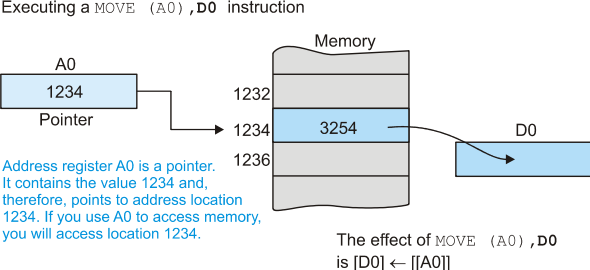
\includegraphics[width=.9\linewidth]{img/indirect-addressing.png}
\caption{Indirect Addressing in Assembly (by Alan Clements)}
\end{figure}
\end{frame}

\begin{frame}[label={sec:orgheadline47}]{Heap Access}
Pointer also provides a way to manage dynamic storage on \emph{heap}.

\begin{description}
\item[{Heap Dynamic Variables}] Variables that are dynamically
allocated from the heap.  They are often \emph{anonymous variables}
(no identifiers associated with them) and thus can be
referenced only by pointer or reference type variables.
\end{description}
\end{frame}

\begin{frame}[label={sec:orgheadline48}]{Pointer Operations}
Two fundamental pointer operations are needed
\begin{description}
\item[{Assignment}] set a pointer variable's value to some useful
address.
\item[{Dereference}] Takes a reference through one level of
indirection, i.e., get the value referenced.
\end{description}
\end{frame}

\begin{frame}[fragile,label={sec:orgheadline49}]{Pointer Assignment}
 \begin{enumerate}
\item A pointer may be initialized through the allocation mechanism,
whether by operator or built-in subprogram

\begin{minted}[]{cpp}
int main() {
  int* a = new int{3};           delete a;
  char* b = (char*) malloc(3);   free(b);
}
\end{minted}

\item In the case of indirect addressing, an explicit operator or
built-in function is needed to get the address of variables not
on heap.

\begin{minted}[]{cpp}
int main() {
  int a = 3;                    // on stack, not heap
  int* b = &a;                  // & to get address of a
}
\end{minted}
\end{enumerate}
\end{frame}

\begin{frame}[label={sec:orgheadline50}]{Pointer Dereference}
When a pointer appears in an expression, it may be interpreted as
\begin{itemize}
\item a normal scalar value, or
\item a value to which is points to, i.e., indirect addressing resulted
by dereferencing the pointer..
\end{itemize}


\begin{figure}[htb]
\centering
\includegraphics[width=.9\linewidth]{img/pointer-deref.pdf}
\caption{Pointer Dereferencing}
\end{figure}
\end{frame}

\begin{frame}[fragile,label={sec:orgheadline51}]{Pointer to Record}
 The syntax may vary.  The following is the syntax for \texttt{C++}.

\begin{minted}[]{cpp}
struct point {
  int x, y;
};

int main() {
  point* p = new point;
  (*p).x = 3;
  p->y = 4;
  delete p;
}
\end{minted}
\end{frame}

\begin{frame}[fragile,label={sec:orgheadline52}]{Pointer Headache}
 \begin{description}
\item[{Dangling Pointer}] Contains the address of a heap-dynamic
variable that has been deallocated.
\end{description}


\begin{minted}[]{cpp}
int main() {
  int* a = new int{3};
  int* b = a;
  delete a;                     // now b is dangling
  delete b;                     // ERROR! Double free!
}
\end{minted}
\end{frame}

\begin{frame}[fragile,label={sec:orgheadline53}]{Pointer Headache Cont'd}
 \begin{description}
\item[{Memory Leakage}] An allocated heap-dynamic variable that is no
longer accessible to the user program.
\end{description}


They are are called \emph{garbage}
\begin{itemize}
\item they are not useful for their original purpose, and
\item they also cannot be reallocated for some new use in the program.
\end{itemize}


\begin{minted}[]{cpp}
int main() {
  int* a = new int{3};
  a = new int{4};               // the old memory is lost
}
\end{minted}
\end{frame}

\begin{frame}[label={sec:orgheadline54}]{Pointer Painkiller -- Tombstone}
\begin{figure}[htb]
\centering
\includegraphics[width=.5\textwidth]{img/tombstone.pdf}
\caption{new(ptr1)}
\end{figure}

\begin{figure}[htb]
\centering
\includegraphics[width=.5\textwidth]{img/tombstone1.pdf}
\caption{ptr2 = ptr2}
\end{figure}

\begin{figure}[htb]
\centering
\includegraphics[width=.5\textwidth]{img/tombstone2.pdf}
\caption{delete(ptr1)}
\end{figure}
\end{frame}

\begin{frame}[label={sec:orgheadline55}]{Tombstone Issues}
\begin{itemize}
\item For heap objects, it is easy to invalidate a tombstone when the
program calls the deallocation operation.
\item For stack objects, the program must be able to find all
tombstones associated with objects in the current stack frame
when returning from a subroutine.
\end{itemize}

Tombstone is expensive, both in time and in space.  Time overhead
includes
\begin{itemize}
\item creation of tombstones,
\item checking for validity on every access, and
\item double indirection.
\end{itemize}


Tombstone is easy for \emph{storage compaction} because of double
indirection.
\end{frame}

\begin{frame}[fragile,label={sec:orgheadline56}]{\texttt{C++} Pointer Wrapper}
 \begin{itemize}
\item For small programs, it is OK and to stay with native pointer.
\item For large programs, use \texttt{shared\_ptr}, \texttt{unique\_ptr} and
etc. declared in \texttt{<memory>} from \texttt{C++} STL.
\end{itemize}


\begin{minted}[]{cpp}
#include <memory>
using namespace std;

int main() {
  shared_ptr<int> a{new int{3}};
  shared_ptr<int> b = a;
  b = nullptr;
}
\end{minted}
\end{frame}

\begin{frame}[fragile,label={sec:orgheadline57}]{Reference}
 \begin{description}
\item[{Reference type}] Similar to a pointer, with one fundamental
difference: a pointer refers to an address in memory, while a
reference refers to an object or a value in memory.
\end{description}


Reference type in \texttt{C++} has the following features
\begin{itemize}
\item It is an \emph{implicitly dereferenced} \emph{constant} pointer.
\item Must be defined when declared since it is constant.
\item May not be set to reference other variables since it is
implicitly dereferenced.
\end{itemize}
\end{frame}

\section{Miscellaneous Type Issues}
\label{sec:orgheadline66}

\begin{frame}[fragile,label={sec:orgheadline59}]{Type Checking}
 \begin{description}
\item[{Type Checking}] The activity of ensuring that the operands of an
operator are of \emph{compatible types}.
\item[{Compatible Type}] A compatible type is one that either is legal
for the operator or is allowed under language rules to be
implicitly converted (coercion) by compiler-generated code (or
interpreter) to a legal type.
\item[{Type Error}] The application of an operator to an operand of an
inappropriate type.
\end{description}


\begin{minted}[]{cpp}
int main() {
  int a = 1.2;
  float b = 1.2 + a;
  int* c = a;                   // WRONG!!
}
\end{minted}
\end{frame}

\begin{frame}[fragile,label={sec:orgheadline60}]{Strong Typing}
 \texttt{C} is called both \emph{strong typed} and \emph{weak typed} by different
authors.

\begin{itemize}
\item An example for a statically, but weakly typed language is C. (\href{http://compilers.iecc.com/comparch/article/95-10-071}{link})
\item LISP engines \ldots{} are themselves generally written in strongly
typed languages like C\ldots{} (\href{http://lists.tlug.jp/ML/0010/msg00352.html}{link}).
\item In a weakly typed language such as C\ldots{} (\href{http://www-plan.cs.colorado.edu/diwan/5535-99/hw-6-soln.html}{link})
\end{itemize}
\end{frame}

\begin{frame}[fragile,label={sec:orgheadline61}]{Static and Dynamic Typing}
 \begin{description}
\item[{Static Typed}] Variable Type is known at compile time.
\item[{Dynamic Typed}] Variable Type is known at runtime.
\end{description}

\begin{columns}
\begin{column}{0.5\columnwidth}
\begin{block}{Static Typing}
\begin{minted}[]{cpp}
#include <string>
#include <iostream>

void silly(int a) {
  if (a > 0) std::cout << "Hi";
  else std::cout << 5.3 + "3";
}
int main() { }
\end{minted}
\end{block}
\end{column}

\begin{column}{0.5\columnwidth}
\begin{block}{Dynamic Typing}
\begin{minted}[]{python}
def silly(a):
    if a > 0:
        print 'Hi'
    else:
        print 5.3 + '3'

silly(1)    # PASSES
silly(-1)   # WRONG
\end{minted}
\end{block}
\end{column}
\end{columns}
\end{frame}

\begin{frame}[label={sec:orgheadline62}]{Type Equivalence}
\begin{description}
\item[{Name Equivalence}] Two variables have equivalent types if they
are defined either in the same declaration or in declarations
that use the same type name, i.e., they can be represented by
the same syntax tree with the same labels.
\item[{Structural Equivalence}] Two variables have equivalent types if
their types have identical structures, i.e., replace the named
types by their definitions and recursively check the
substituted syntax tree.
\end{description}
\end{frame}

\begin{frame}[fragile,label={sec:orgheadline63}]{Structure Equivalence Issue}
 \begin{itemize}
\item What parts constitute a structural difference?
\begin{itemize}
\item Storage: record fields, array size
\item Naming of storage: field names, array indices
\item Field order
\end{itemize}
\begin{minted}[]{cpp}
struct point1 { int x, y; };
struct point2 { int a, b; };
int a[5];
int b[5];
\end{minted}

\item Intentional vs incidental structural similarities.
\end{itemize}
\end{frame}

\begin{frame}[fragile,label={sec:orgheadline64}]{Name Equivalence Issue}
 Argument: They're different because the programmer said so; if
they're the same, then the programmer won't define two types!!

So what about \emph{alias}?

\begin{minted}[]{cpp}
struct point1 { int x, y; };
typedef point1 point2;
\end{minted}
\end{frame}

\begin{frame}[fragile,label={sec:orgheadline65}]{\texttt{C++} Type Equivalence}
 Both name and structure equivalence exist.

\begin{itemize}
\item Name equivalence is used for \texttt{struct}, \texttt{enum} and \texttt{union}.
\item Structure equivalence is used for other \emph{non-scalar} types.

\begin{minted}[]{cpp}
void foo(int a[]) { }

int main() {
  int a[5];
  int b[10];
  int* c = new int [3];
  foo(a); foo(b); foo(c);
  delete[] c;
}
\end{minted}
\end{itemize}
\end{frame}

\section{Conclusion}
\label{sec:orgheadline68}

\begin{frame}[label={sec:orgheadline67}]{Summary}
Data type influences PL's usefulness and convenience.

\begin{itemize}
\item Most PL include primitive data types, i.e., numeric, character,
and Boolean.
\item Array (or equivalent) is essential in most PL's.
\item Most PL provides user-defined types, e.g., record, for data
abstraction.  Discussed further in OOP.
\end{itemize}
\end{frame}
\end{document}
